%% LyX 2.1.2.2 created this file.  For more info, see http://www.lyx.org/.
%% Do not edit unless you really know what you are doing.
\documentclass[english]{article}
\usepackage[T1]{fontenc}
\usepackage[utf8]{luainputenc}
\usepackage{array}
\usepackage{longtable}
\usepackage{float}
\usepackage{graphicx}
\usepackage{setspace}

\makeatletter

%%%%%%%%%%%%%%%%%%%%%%%%%%%%%% LyX specific LaTeX commands.
%% Because html converters don't know tabularnewline
\providecommand{\tabularnewline}{\\}

%%%%%%%%%%%%%%%%%%%%%%%%%%%%%% User specified LaTeX commands.
\usepackage{titlesec}
\setcounter{secnumdepth}{5}
\usepackage{enumitem}
\setitemize{nolistsep}
\newcommand{\planlist}{\setitemize{nolistsep}}

\makeatother

\usepackage{babel}
\begin{document}

\title{HuddleLamp - Interim Report}


\author{Jose Kalladanthyil}

\maketitle
\pagebreak{}

\tableofcontents{}

\pagebreak{}


\section{Introduction}
\begin{quote}
“Science fiction writers foresee the inevitable, and although problems
and catastrophes may be inevitable, solutions are not.” (Isaac Asimov) 
\end{quote}
\begin{singlespace}
For an idea to be envisioned and come to fruition someone has to dream
it first. People that dream the biggest and challenge the boundaries
of our imagination are science fiction writers and moviemakers. Various
technology advances and human feats were shown, or animated in the
movies were then made into reality by various companies. I.e. smart
watches were a popular gadget for various detective movies especially
James Bond Movies. Smartphones was also popular in movies like matrix,
and James bond movies. Another gadget that was very popular in a lot
of mainstream movies was an interactive table, like the one in Star
Trek. Where a lot of people can collaborate and contribute sitting
around a table. Even though the idea was exciting and intrigued a
lot of people, this has not been as popular as the other gadgets because
of the high production cost which lead to even higher retail price
of this product. 
\end{singlespace}

HuddleLamp \cite{HuddleLamp} is a project to compete with the fact
that interactive tables are quite expensive; making it is inaccessible
for some everyday consumers such as schools, public libraries, community
centers etc. HuddleLamp aim to use the multitude of unused tablets
and smartphones, which people have lying around and create an ad-hoc
interactive table by using a novel sensing and detection method to
deduce where the devices are and what they should be shown. 

HuddleLamp proposes to use some of the cheaper off-the-shelf products
like a webcam, and a lamp to create a cheaper interactive table that
anyone could use. HuddleLamp proposes to use a hybrid sensing approach
that uses RGB and depth data, that can be obtained from sophisticated
webcams, which can detect and identify mobile displays on tables and
track their positions and orientations \cite{HuddleLamp}. The project
devised a way that multiple devices can interact with each other in
such a way that they all serve as one seamless multi-device user interface. 

Some of the main advantages of HuddleLamp were the face that you seamless,
ad-hoc way of adding devices to the UI. Using HuddleLamp, users can
add or remove displays and reconfigure them in space without the need
of installing any software or attaching markers. Placing them below
the camera implicitly does the setup and pairing of devices. Opening
a URL on the device and making it visible to the camera adds the new
device to the “Huddle”. The camera also tracks the hand movements
of the user, enabling interactions between the devices. 

The simplicity in adding a device to the table means users are not
constrained by having specific devices or requiring them to download
particular apps. This also means collaboration can occur on tables
that are cluttered with other objects likes pens and pencils. There
are 2 main components that’s required for HuddleLamp; a camera, they
suggest Creative Senz3D camera, and a desk lamp, both are relatively
inexpensive components compared to an interactive table. 

However there are some deficiencies in this improvisation to make
an interactive table. At the time of writing, the project has not
release a public version of their software. The developer’s version
requires you to connect a computer with the webcam, which does most
of the grunt work in term tracking devices. In this architecture of
HuddleLamp, this does all the resource intensive tasks so if it’s
not a really powerful computer, there are lagging experiences by the
users. The fact that to set this interactive table up you need to
connect a lamp up to a computer means that the whole setup is not
very portable. The size of the interactive part of the table is constrained
by how high up the camera is, from the surface of the table. The use
of camera means users’ arms and hands can sometimes impede the detection
and tracking of devices during moving or touching the devices. 

For these reasons, I propose to create an app, which can communicate
and collaborate with other mobile devices running the same app nearby.
I envision using Bluetooth Low energy technology that came to the
fore over the recent years and the advancement done by Apple in iBeacon
technology\cite{Maisto2013}, and creating an indoor positioning algorithm
around a table. 

This solution can clearly get rid off the camera used by HuddleLamp
to make the whole system much more portable. I want to place 3 iBeacon
nodes around the table and use trilateration algorithm. Its similar
to algorithms used in movies for tracking people using the phone signals.
The web architecture implementation would ensure that all the devices
would have a synchronised data showing ensuring collaboration between
the devices. 

This idea in turn has several challenges that need to be overcome.
The main challenge is the fact that Bluetooth technology is not designed
exact positioning. Even though the idea is theoretically possible
and also there exist libraries, which helps in this scenario. Advanced,
sophisticated algorithms needs to be created which can factor the
error that is prone to show up. Bluetooth signal is just a 2.4 GHz
radio wave and as such is susceptible to factors like absorption,
diffraction, interference and multipath propagation. Therefore to
achieve more than 5-6m accuracy using trilateration, you need really
advanced noise cancelling algorithms. 

Over the course of this project I wish to investigate into the possibility
of using BLE technology for accurate positioning. Evaluation will
be predominantly through comparison with HuddleLamp, and creating
my own tests to compare with the HuddleLamp implementation. 

Another big challenge that has to be overcome is the lagging experienced
by the users of the HuddleLamp. Some of the main culprits for the
lagging in the HuddleLamp project were the processing power of the
computer used and the delay of transferring information through the
web sockets. Using the power of cloud computing and scalable cloud
applications like Heroku should ensure that the lagging would stay
to a minimum. 

One of the big advantages of the hybrid sensing system employed by
HuddleLamp was the ease to track the mobile devices on the table.
This is another aspect that I would require to replicate using BLE
technology. I have decided to overcome this by using the sensors like
accelerometer and compass on the devices and dead reckoning. Dead
reckoning is the process of calculating one's current position by
using a previously determined position, or fix, and advancing that
position based upon known or estimated speeds over elapsed time and
course. \cite{DeadReckoning}


\section{Background}

There are a lot of very important decisions that needs to be taken
before the implementation of the product. There are a wide choice
of options for each aspect of product such as positioning, implementation
language, benchmarking. Over the course of this section we will go
through some of the similar work done by other research labs. Also
go through some of the options that need to be narrowed down, where
we will see the advantage and disadvantage for the choices and then
pick the method we will be implementing. 


\subsection{Related Work}

Interactive table is by no means a new idea. A lot of research has
been undertaken to find a simple suitable solution for the problem. 


\subsubsection{LightSpace }

One of the companies that do a lot of research into this area is Microsoft.
One of their researches is into a system called LightSpace. LightSpace
is a small room installation designed to explore a variety of interactions
and computational strategies related to interactive displays and the
space that they inhabit \cite{Wilson2010}. This was a research that
investigated into touch sensitive interactive displays which was built
using cameras and projectors to simulate a fully virtual 3D environment.
As you can see from FIGURE 1 LightSpace is not a portable design,
aimed at turning a whole room into an interactive space. It is a more
sophisticated implementation with larger set of use cases. Including
picking and dropping virtual object. It gives a more augmented reality
environment. There are other limitations to LightSpace, like it can
only emulate interactive display features on flat, static shapes that
are designated beforehand.

\begin{figure}[H]
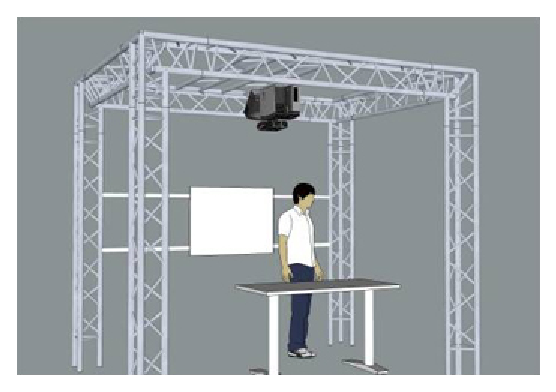
\includegraphics{LightSpace_configuration}\protect\caption{LightSpace Configuration}
\end{figure}



\subsubsection{Beamatron }

Another research undertaken by Microsoft is Steerable displays \cite{Wilson2012}.
It uses a motorized platform to orient a projector to display graphics
at any point in the room. It is quite similar to the LightSpace research
we discussed previously, however the Beamatron can project graphics
in the user’s hand, and follow the user as they move about the room.
It uses a depth camera to calculate the live changes in the room such
as following a user’s hand. It discusses how we can move 2D graphics
using gestures. 


\subsubsection{ConnecTable }

ConnecTable is one of the earlier concepts for interactive table using
multiple devices \cite{Tandler2001}. It’s a mobile, context aware
information appliance, which uses a pen-based interaction. It also
has the capability of extending its display area to merge multiple
ConnecTable together to form one large display. There are primary
mode of interaction with ConnecTable is the pen based method. Sensors
are also building onto the ConnecTable, allowing the interpretation
of physical actions in the real world, mapped to an action on the
table depending on the software used. ConnecTable is a Roomware component.
Roomware is a concept where lots of multiple objects in a room could
interact with each other in a way that they would be able to provide
information of what is happening in the room.\cite{Roomaware}


\subsection{Radio Frequency Signal}

One of the biggest decisions that need to be taken for our implementation
is the type of Radio Frequency signal (RF) we are going to use for
our positioning. There are quite a few mainstreams RF widely used,
such as Wi-Fi, Near Field Communication (NFC), Bluetooth, Bluetooth
Low Energy (BLE) also known as Bluetooth smart. In this section we
are going to look at the advantages and the disadvantages of these
RF signals. 


\subsubsection{Wifi }

Wi-Fi is one of the most used RF signals out there. It is used for
computer networking using 2.4 GHz UHF and 5 GHz SHF ISM radio bands.
The services provided are also numerous, from consulting web pages
to watching on demand video sequences. 

One of the biggest advantages of Wi-Fi is the fact that it’s widely
used. Almost all location has Wi-Fi now, which means the setup cost
and maintenance cost of Wi-Fi would be cheap. It also has the ability
to transfer complicated data between its Access point (AP) and the
mobile devices, making it highly adaptable. 

Wi-Fi has been used for indoor positioning before by various research
groups. Two positioning techniques have been used for this research
called Signal Strength Cartography and Wave propagation. Signal Strength
Cartography is a reference-based system where you map the area offline
with coordinates and the strength of the Wi-Fi signal. Then when you
are trying to locate a device use the coordinates and the strength
to work out where exactly the device is. There are two main steps
for this mapping, an offline mapping step, which could be done either
by simulation or manually using measurements, and an online positioning
step, which could be done either using a probabilistic method or deterministic
method. 

Wave propagation approach is a mathematical attempt at finding the
distance between the device and the transmitter by finding a relation
between the distance and the signal strength. By using at least 3
AP we can use wave propagation and trilateration to work out the position
of the device. 

However there are various disadvantages of using Wi-Fi to work out
positioning of the devices. There are usually only one AP per location,
however we would require more than one, to get more accurate positioning
of the devices. Wi-Fi works mainly by sending signals in channels,
so having more than one Wi-Fi AP in a location could produce congestion
in channels, which would create interference. Wi-Fi also has a higher
power consumption. This is because of the larger range in which Wi-Fi
sends out its signal. 

There is hope for using Wi-Fi as the main Radio frequency for our
product in the future after the Wi-Fi Standards agency brings out
Wi-Fi -aware. Which is proximity based discovery system. Introduction
of this system could mean that you don’t require any extra AP, and
the devices could interact with each other without any outside help. 


\subsubsection{Global Positioning System (GPS)}

GPS is one of the most widely used features in our devices. Over the
past few years the use of GPS has increased significantly due to the
increasing social network activity. Nowadays almost every app that
we use through our mobile devices request for GPS access which shows
how much it has come forward. GPS is a space based navigation system
using the satellites. The Department of Defence of USA, using the
24 satellites already in orbit, initially introduced it. 

GPS satellites transmit data continuously, which contains their current
time and position. A GPS receiver listens to multiple satellites and
solves equations to determine the exact position of the receiver and
its deviation from true time. At a minimum, four satellites must be
in view of the receiver in order to compute four unknown quantities
(three position coordinates and clock deviation from satellite time). 

The main advantage of GPS is that it’s widely available. Almost all
devices have a GPS receiver on it. It also has a very large range.
However it is not a viable option for us because of the fact that
the signal comes from outer space and our devices are usually indoors.
GPS like any radio frequency signal is prone to absorption and diffraction
by the roof and walls in the building. GPS also has high power consumption.
GPS tends to be not very accurate, averaging \textasciitilde{}10m
which would make it unviable for our use. 


\subsubsection{Bluetooth}

Classic Bluetooth, usually known as Bluetooth, was the codename for
a project by Special Interest Group (SIG), collaboration between some
major companies, like Ericsson, Intel, and Nokia. Bluetooth was invented
for short-range wireless communication with devices. Bluetooth uses
radio signals in the 2.4 GHz range to transmit data. This range is
globally license free range; therefore there is no extra cost for
deployment. Bluetooth is not targeted any specific application, therefore
a multitude of applications has used Bluetooth in various different
ways from transferring files to streaming songs.\cite{ChalmersBLE} 

SIG is in charge of the specification of Bluetooth and creating a
roadmap for it going forward. To standardise the form of communication
through Bluetooth, SIG has defined a set of profiles that needs to
be made available by the manufacturer. Devices usually only have a
subset of these profiles enabled. Some of these profiles are: 
\begin{itemize}
\item A2DP Advanced Audio Distribution Profile. Used for Streaming audio. 
\item HFP Hands-Free Profile. Used for hands free kit to make calls in cars 
\item HID Human Interface Device Profile. Provides support for input devices
like keyboards, mice and game controllers.
\end{itemize}
Bluetooth is aimed at applications that require short-range communication
typically few meters. The actual range an application make depends
on the Bluetooth Class the application has and also external circumstances
like absorption, diffraction etc. Bluetooth devices are separated
out into 3 different classes with separate transmission power. The
full picture is shown in Table 1.

\begin{tabular}{|c|c|c|c|}
\hline 
Class & Max Power Output & Max Range & Power Level Control\tabularnewline
\hline 
\hline 
1 & 100 mW & 100 m  & Mandatory\tabularnewline
\hline 
2 & 2.5 mW & 10 m & Optional\tabularnewline
\hline 
3 & 1 mW & 1 m & Optional\tabularnewline
\hline 
\end{tabular}
\begin{table}[H]
\protect\caption{Bluetooth Power class}
\end{table}


Due to the different profiles and more than sufficient range and relatively
low power consumption, Bluetooth shows considerable potential to be
used as our Radio frequency signal for our positioning. However they’re
some aspects of it, which makes it difficult for Bluetooth to be used.
The main problem is the security constraints of Bluetooth, which requires
the devices to go through a pairing process with each other. 

In Bluetooth technology a device could take either the master role
or the slave role. Before the devices can communicate with each other
they have to discover each other and specify which profile they are
going to use. Pairing is done by: 
\begin{enumerate}
\item Master devices continuously broadcast “inquiry messages”
\item These messages will be picked up by nearby devices that are “discoverable” 
\item These devices will respond with a message containing their name, profiles
they support and other technical details. 
\item Using these details the master device can establish a connection with
the correct profile 
\end{enumerate}

\subsubsection{Bluetooth Low Energy (BLE)}

BLE is a relatively new technology, which came out in 2010 with the
new specification for Classic Bluetooth 4.0. BLE was introduced for
devices that are predominantly used for monitoring and control, like
sensors values and control commands, where there is no need for large
amount of data transfer.


\paragraph{Modes\protect \\
}

One of the biggest improvements introduced for BLE that is not there
for Bluetooth is the addition of the new mode. This new mode takes
away the necessity for pairing to exchange data. In this “broadcast”
mode the device can send data in the advertisement channel. There
are 4 different modes in BLE\cite{ChalmersBLE} : 
\begin{description}
\item [{Central}] : Similar to the Bluetooth master role, can have multiple
connections. 
\item [{Peripheral:}] A device can only have one active connection with
the central mode 
\item [{Broadcaster}] : Where you send data in the advertisement channel
\item [{Observer:}] Where you listen to the advertisement channel
\end{description}

\paragraph{Scanning\protect \linebreak{}
}

Another big improvement BLE has brought is the ability to discover
other devices in two different modes. BLE enabled devices can now
passively and actively scan for connectable devices.
\begin{itemize}
\item Passive scanning - a central device listens to the advertising channel
passively to capture all the packets transmitted by connectable devices 
\item Active scanning - a central device listen for advertisement packets
and when it receives the packet, it checks whether the sender is connectable
through looking at the mode. If it is then a scan request packet is
send to gain more information.
\end{itemize}
Devices may advertise as seldom as once every 10 seconds or as fast
as every 20 millisecond. 


\paragraph{Range\protect \\
}

Similar to the Classic Bluetooth, the range of BLE is determined by
the transmitting power and the interference that it might experience.
BLE has a transmitting power up +10dBm, which gives it a range of
300m theoretically. However BLE usually use a power of 0dB or less
which gives it a range of about 50m{[}link 9{]}. Even though BLE is
meant to have low-energy consumption, it has a bigger range than Classic
Bluetooth under maximum power due to smaller packet size. 


\subsection{Positioning algorithms}


\subsubsection{Ecolocation}

Ecolocation is a RF based location algorithm \cite{KiranYedavalliBhaskarKrishnamachariSharmilaRavula2005}.
It uses the sequence of received signal strength RSS from nearby reference
nodes with known locations, to find the location of the unknown node.
By ordering the reference nodes by their distance we are able to map
different regions of the space to their unique signature.
\begin{description}
\item [{Training~phase}] During the training phase, we divide the area
(the table), where the device is going to be, into segments. We go
through these segments and detect the RSS signal from all of the reference
nodes and store them to a database. 
\item [{Online~phase}] Online phase is when an unknown device in in the
area and we want to know its location. The device collects the RSSI
information from the reference nodes and compares it to the stored
information in the database, to get best match or get geometric median
of the K-closest values, to work its location. 
\end{description}

\subsubsection{Trilateration}

Trilateration is one of the oldest and most recognisable methods of
estimating location of an object. We use a minimum of three reference
nodes and the distance between them and the device to work out the
position of the device. The reference nodes are used as centres of
circles and the distance is used as the radius of those circles. The
point of intersection of those three circles is the relative or the
actual position of the devices depending on whether the location of
the reference nodes is known. In most cases of position systems the
reference nodes are beacons or access points. The distance can be
measured using RSS or time of flight (TOF), time taken for the signal
to reach the device. These measurements combined with the coordinates
of the beacons can form the basis of trilateration.


\paragraph{Signal Based Position}

From previous work done for indoor positioning we know that many different
signal characteristics could be taken into account to determine the
position of the device. Some of these characteristics are:
\begin{description}
\item [{Angle~of~Arrival~(AoA)-}] Angle of Arrival compares the direction
from which the different signals arrive at the devices. Using the
received angle, we can determine it direction from which the signal
came from. If we have multiple signals coming to the device, we can
find the exact location of the device by looking at where the lines
intersect. We need a minimum of two reference points and two angles
to work out the correct position. There are many difficulties with
the method; the device would need to know its own orientation to work
out the correct angle. The sensor that detects the signal needs to
be very advanced (more advanced than the ones usually found on a device. 
\item [{Time~of~Arrival~(TOA)}] - By using the time of arrival of the
signal and the time of sending of the signal and the medium in which
it travelled through we can work out the distance of the devices from
reference nodes. This coupled with a database of known travelling
time we can work out where the device is. This would however mean
we would have to keep a database of results and wont be very portable.
\item [{RSSI~-~Based}] -Similar to trilateration, the device can use
the Received Signal Strength Indicator (RSSI) to work out distance
from the reference nodes. Any device with a proper network adapter
can work out the RSSI value.
\end{description}

\subsubsection{Filter~Methods}

Filter based positioning uses mathematical methods to estimate the
positioning of the device, using some given observations from the
system. The observation can be anything from distance to references,
previous estimated position or sensor inputs such as a compass or
gyroscope. This technique has been used for many different applications.
Its very helpful because it allows us to incorporate many other sources
of data that we could potentially has for the system. A good example
of this is presented in \cite{rag}, where they use ultrasound as
the radio frequency signal and combine it with odometer reading to
get a better accuracy for their tracking ability. 

A particle filter work by continuously generating thousands of particle
at random during runtime. For positioning, these particles represent
the location that the device could be. We can calculate the distance
to the reference beacons for each particle. By using the observer
value from the device we can eliminate and filter out those particles
that are unlikely to be the correct location. We then use the remaining
particles to calculate an estimate for the position of the device.
The filtering is done by assigning weights to the entire particle
depending on how reasonable the particle values are according to the
observed value. Gradually, most of the particles will have negligible
weight and therefore would not affect the estimation while some particles
with significant weights will remain affecting the estimated value
significantly. To avoid this problem we resample the higher weight
particles while particles with negligent weights are discarded. During
the initial step we uniformly distribute the particles around the
map, later particles and discarded or saved depending on the filtering
method. Two of the most commonly used filter methods are Kalman Filter
\cite{Kotanen2003} and Mote Carlo Filter\cite{MonteCarlo}. 


\section{Project Plan}

{\planlist 

\begin{longtable}{|>{\raggedright}p{0.13\textwidth}||>{\raggedright}p{0.3\paperwidth}||>{\raggedright}p{0.15\paperwidth}|}
\hline 
Date & Target & Fall Back Milestone\tabularnewline
\hline 
\hline 
30- Jan & \begin{itemize}
\item Finish Interim Report,
\item Finish research into frameworks
\item Identify the frameworks to be used
\item Learn the frameworks\end{itemize}
 & \tabularnewline
\hline 
\hline 
17 - Feb & \begin{itemize}
\item Implement the basic bluetooth listening app
\item use the app to get data for evaluation on distance
\item Start implementing trilateration\end{itemize}
 & \tabularnewline
\hline 
\hline 
1- March & \begin{itemize}
\item Finish implement trilateration
\item Get data by testing it on a grid to get the error in trilateration
\item Start adding dead reckoning information and start filtering methods
\item finished background for the full report\end{itemize}
 & \tabularnewline
\hline 
\hline 
15- April & \begin{itemize}
\item finish implementing filtering methods
\item get error rate adjust the filtering method to get it working
\item Start implementing the mobile app with a picture and moving on picture
to get it working
\item finish evaluation of the full report including tables charts and diagrams\end{itemize}
 & App that shows a fiteration method ie. a rectangle with dots to show
the position of the app!\tabularnewline
\hline 
\hline 
30-April & \begin{itemize}
\item Finish evaluation section for the report 
\item Get background and evaluation checked by tutor\end{itemize}
 & \tabularnewline
\hline 
\hline 
15- May & \begin{itemize}
\item Finish moving picture app 
\item Do other parts of the report\end{itemize}
 & Moving picture app similar to where is waldo type app\tabularnewline
\hline 
\hline 
30-May & \begin{itemize}
\item Finish the report 
\item add gesture control to the app\end{itemize}
 & gesture control app\tabularnewline
\hline 
\hline 
15-June & \begin{itemize}
\item Be at a stage where report needs to proof read and checked
\item Finish the gesture control
\item final hacking session to get the app presentable\end{itemize}
 & \tabularnewline
\hline 
\hline 
30-June & \begin{itemize}
\item Everything should be finished\end{itemize}
 & \tabularnewline
\hline 
\end{longtable}

}


\subsection{Potential Extentions}

There are various extensions I would like to do including:
\begin{itemize}
\item Finish the gesture controls
\item Make it more of a platform so that people can create a workspace they
want
\item Have some in app workspaces like blank drawing page, casino games
\item Have the ability for the picture app to import pics from library
\end{itemize}

\section{Evaluation Plan}

As you can see from the background research, a lot of companies and
individuals have done various researches into creating an interactive
table. A lot of research has also been undertaken in the topic of
indoor positioning, especially with Bluetooth and BLE. Therefore there
is a lot of information about Bluetooth and Trilateration and filtering
techniques. I will be undertaking a research in the use of Bluetooth
for positioning in a smaller area. Where I believe the error in sensing
would be much smaller. Basic sensing of Bluetooth signalling augmented
with odometer data and filtering techniques would give me positioning
information to a quite a good accuracy level. 

There are several ways for me to evaluate the research I have done
and the accuracy of the techniques I have used. As you can see from
the progress plan I aim to gather information about distance measurements
through Bluetooth and compare it to real world, physical distance
and calculate the error for it. Another experiment I would do after
that it to work out the error for trilateration and dead reckoning
and create an app, which uses a filtration method like the Monte Carlo
localization filter to gain a confidence level of where the device
is. I would do this by having a large sheet of paper, which would
be divided into a grid and calculating where the device is. All of
this data combined should give me an accurate picture of the sensing
abilities of a device. This should in turn help me build an app where
I can take these error information into account and create a robust
app which should be quite accurate. I am aiming to get as close as
possible to the sub-centimetre range that HuddleLamp was able to achieve
with their implementation. 

Another evaluation experiment I would like to try is a way to benchmark
the loading time. How quickly panning and gesture could be passed
back to the app. It is something I would also evaluate by comparing
it to the HuddleLamp setup I have in the office. Comparison between
the implementation for load times might not be the ideal scenario
since the loading of information in HuddleLamp is subject to the computer
in which the Visual Studio project is running. Different computers
can give different result for this experiment. 

Finally I would also have an evaluation where I would give some users
an opportunity to use the app and see how they do. Then I would try
and do get a questionnaire filled to get their feedback. I would try
and get a wider variety of views including from graphic designers,
students, lecturers etc.


\author{\bibliographystyle{plain}
\bibliography{References1}
}
\end{document}
